\chapter{Introduction}
One of the biggest challenges in modern research is the study and the 
development of humanoid robots. Building a machine that is capable of executing 
the same tasks that the humans do is of fundamental importance for the future 
of our society, freeing people from dangerous and laborious jobs, increasing 
productivity and well-being. The idea of replicating the characteristics of 
the human body has fascinated humanity since the conception of Leonardo's
Robot (1495) by Leonardo Da Vinci \cite{Moran2007TheDaVinciRobot}. Human 
knowledge has advanced so much in the last centuries that the dream of 
building a machine that resembles the human body has finally become true.

This chapter introduces humanoid robots, giving an overview of the technology 
that has been developed in the last decades and a comparison to other robots
such as manipulators and unmanned ground vehicles. The problem of legged 
robot locomotion is then discussed, describing the current state-of-the-art 
research, the modules that allow a 
humanoid robot to safely move inside a specific environment, such as 
localization, mapping, planning and control, and the way they seamlessy work
together in order to realize humanoid gaits.

Even if humanoid robots are nowadays capable of realizing astonishing tasks,
many challenges are yet to be solved before their introduction in our 
society, making them part of our daily life. The goal of this thesis is that 
of studying humanoid robot locomotion in a world known as \textit{World of 
Stairs}, where the environment surrouding the robot is composed of 
horizontal patches located at different heights \cite{ECC19}. This chapter 
concludes by presenting an overview of the thesis, discussing its 
structure and the content of each chapter. 

\section{Humanoid Robots}
General overview, story, comparison with UGV. Importance of humanoid robots 
and applications. Humanoid robots are, more in 
general, legged robots.

Some humanoid robot platforms.

The development of humanoid robots started in 1967 with the WABOT-1
\cite{Kato1973TheWABOT1AI}, shown in Fig. \ref{fig:wabot-1}, created by Waseda
University. WABOT-1 is
the first anthropomorphic robot able to 
walk with its limbs and carry objects with its hands. It was also equipped with 
a vision and a communication system that allowed it to communicate with people 
in Japanese. The most famous humanoid robot is probabily ASIMO
\cite{Sakagami2002TheIntelligentASIMO}, developed by HONDA (Fig.
\ref{fig:asimo}). Its development started in the
1980s and it was preceded by many different version before being presented in
2000.
The last version of ASIMO is tall 130 cm and is able to recognize objects,
gestures, sounds and 
faces, making it able to interact with humans. It is equipped with multiple 
sensors such as laser and infrared that allowed it to autonomously 
navigate. ASIMO is able to walk and run up to a speed of 9 km/h with an 
autonomy of one hour. Another very famous robot is NAO \cite{NAOdesign},
which development has been started by Aldebaran and continued by Softbank after 
its acquisition. NAO (Fig. \ref{fig:nao-v6}) is the official robot used in 
the RoboCup \cite{Kitano1997RoboCup} Standard Platform League, an international
competition that consists in a soccer tournament where the teams are composed 
of 5 robots. The goal of the RoboCup is that of winning against a FIFA
World Cup winner team by 2050. Most recent and advanced humanoid robot 
includes iCub \cite{Sandini2007iCub}, shown in Fig. \ref{fig:iCub}, designed 
by the RoboCub Consortium and built by Italian Institute of Technology,
with the idea of being a research platform for cognitive robotics;
ATLAS (Fig. \ref{fig:atlas}), developed by Boston Dynamics for emergency service
and rescue operations, such as those described by DARPA Robotics Challenge
\cite{Atkenson2018DARPARoboticsChallengeFinals}, illustrated in Fig.
\ref{fig:drc}; Valkyrie (Fig. \ref{fig:valkyrie}), developed by NASA with the 
aim of advancing human spaceflight and extraterrestrial exploration
\cite{Radford2015Valkyrie}.

\begin{figure}
  \centering
  \begin{subfigure}[b]{0.4\textwidth}
    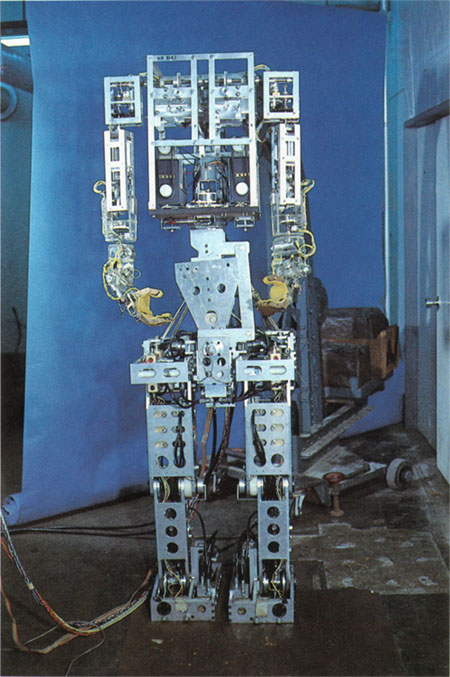
\includegraphics[width=\textwidth]{figures/WABOT-1.jpg}
    \caption{}
    \label{fig:wabot-1}
  \end{subfigure}
  \begin{subfigure}[b]{0.4\textwidth}
    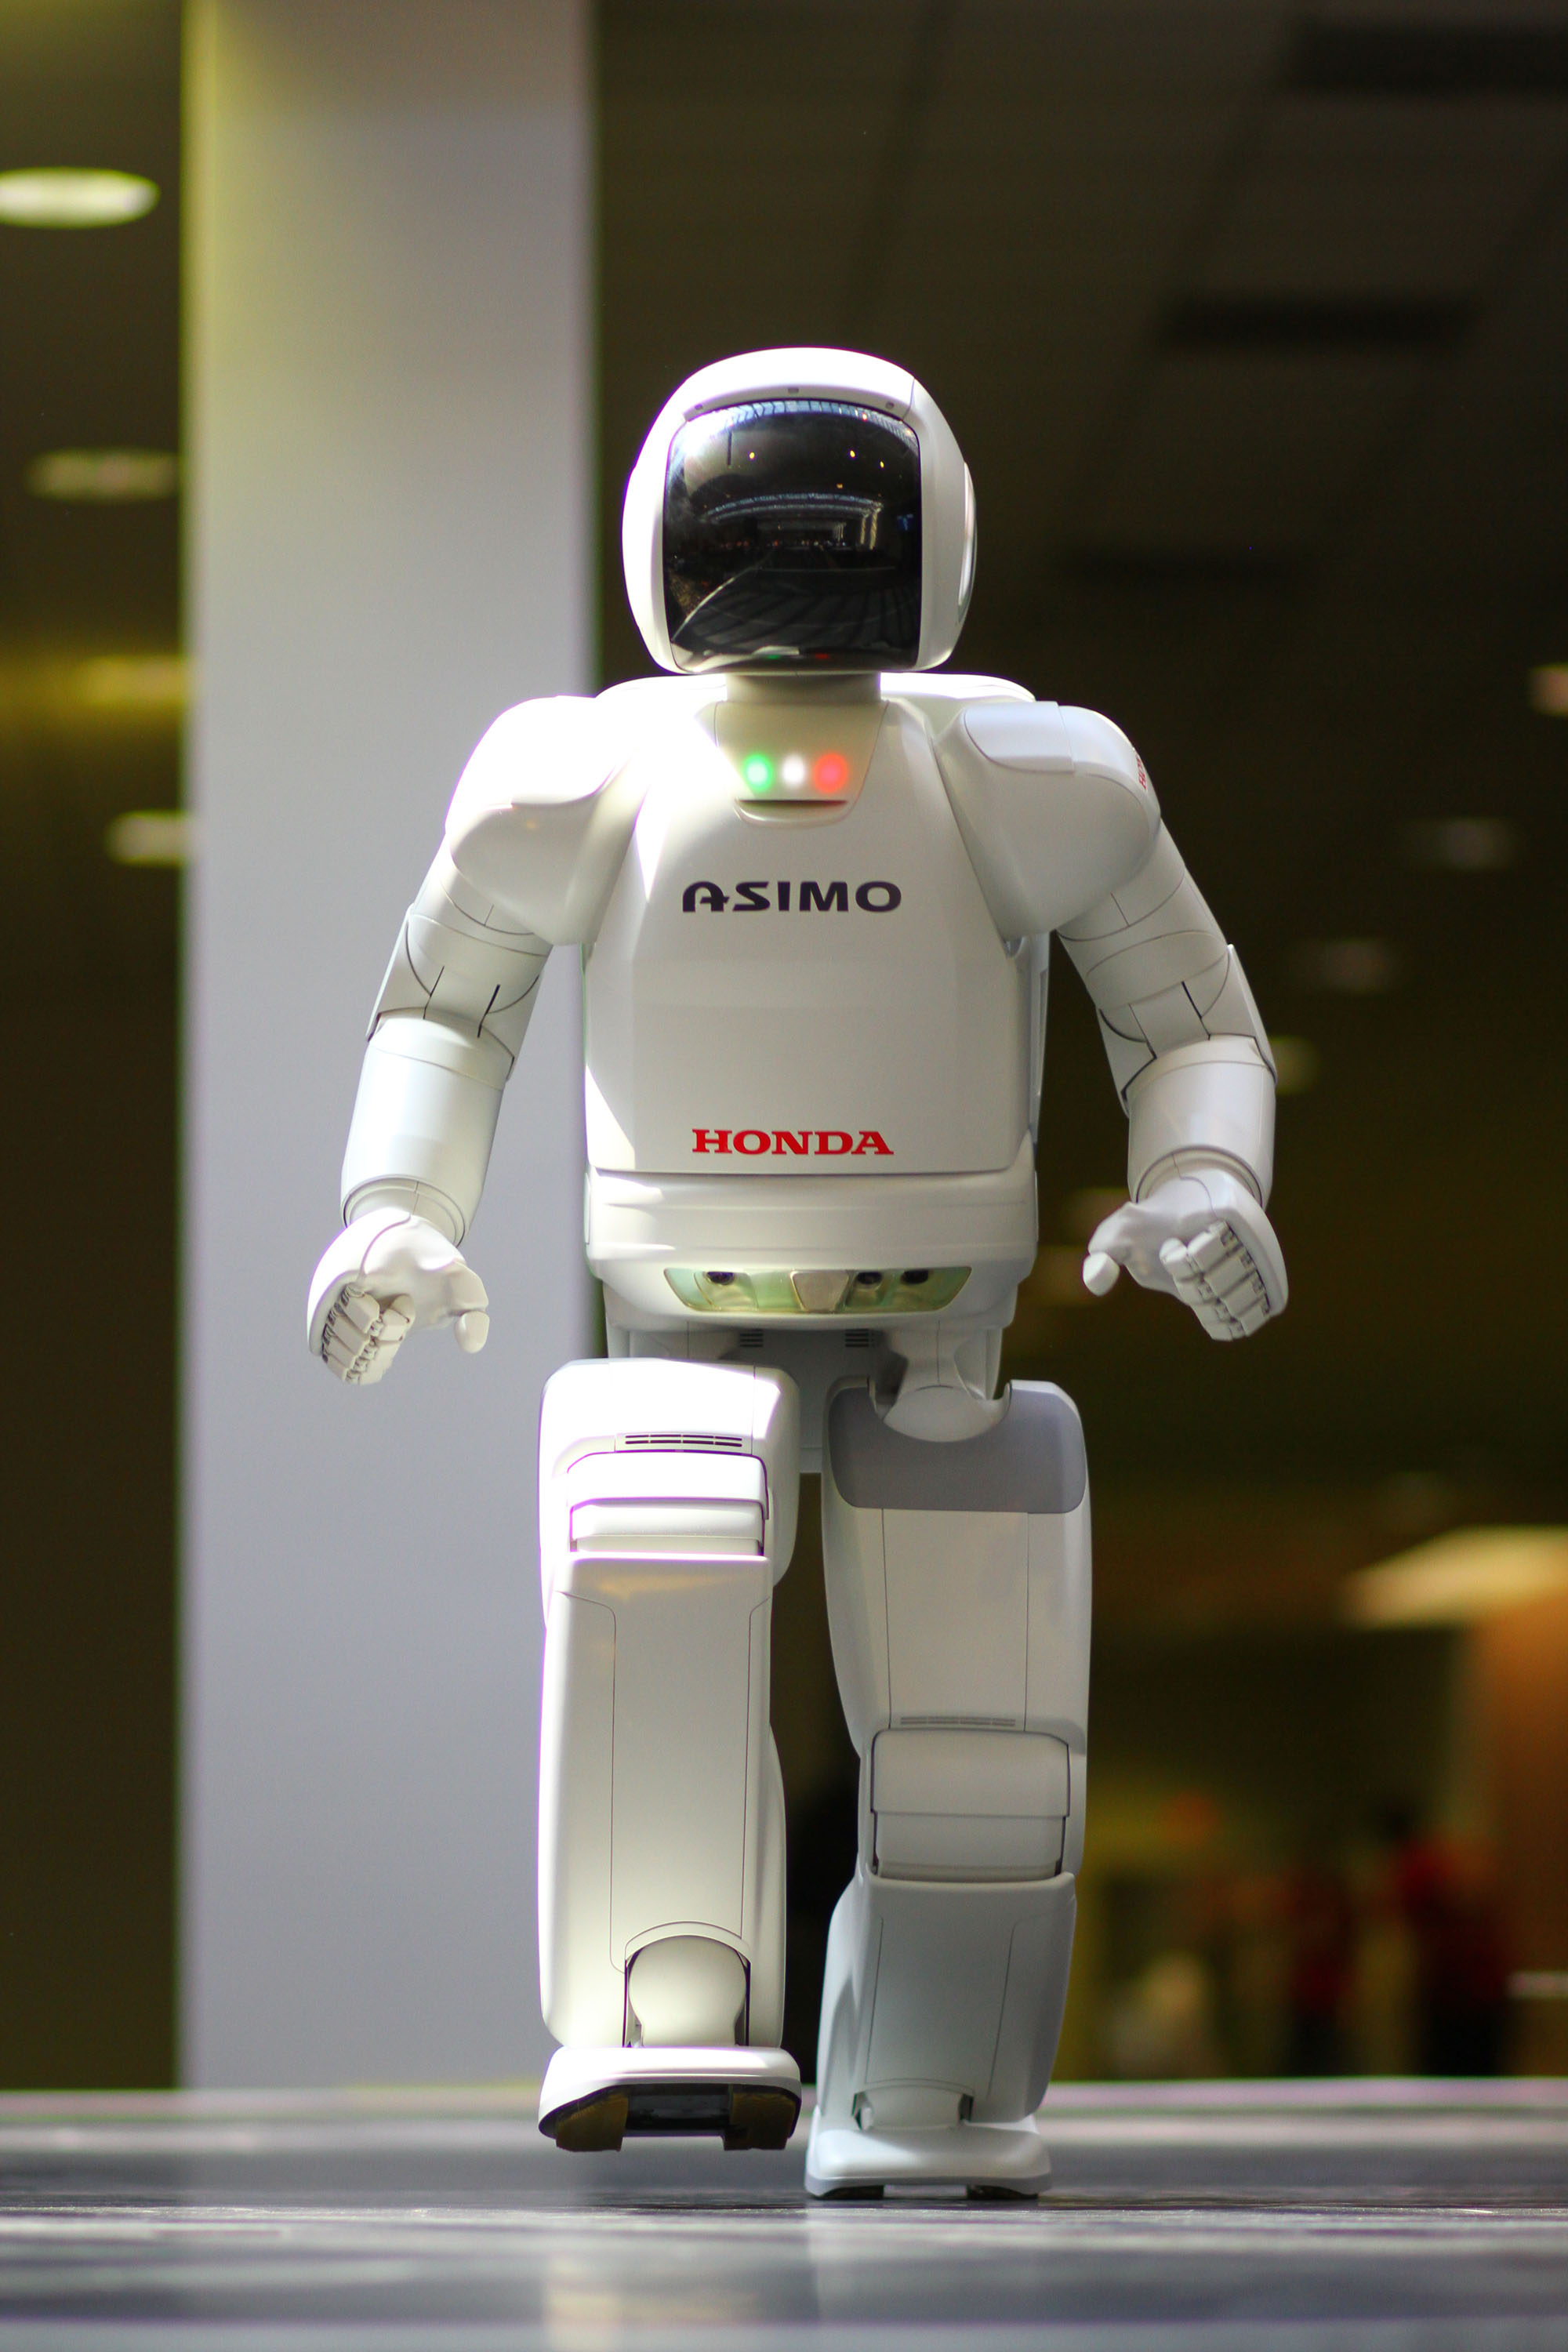
\includegraphics[width=\textwidth]{figures/ASIMO.jpg}
    \caption{}
    \label{fig:asimo}
  \end{subfigure}
  \caption{WABOT-1 \cite{Kato1973TheWABOT1AI} on the left, the first 
      anthropomorphic robot. ASIMO \cite{Sakagami2002TheIntelligentASIMO} on
      the right.}
\end{figure}

\begin{figure}
  \centering
  \begin{subfigure}[b]{0.4\textwidth}
    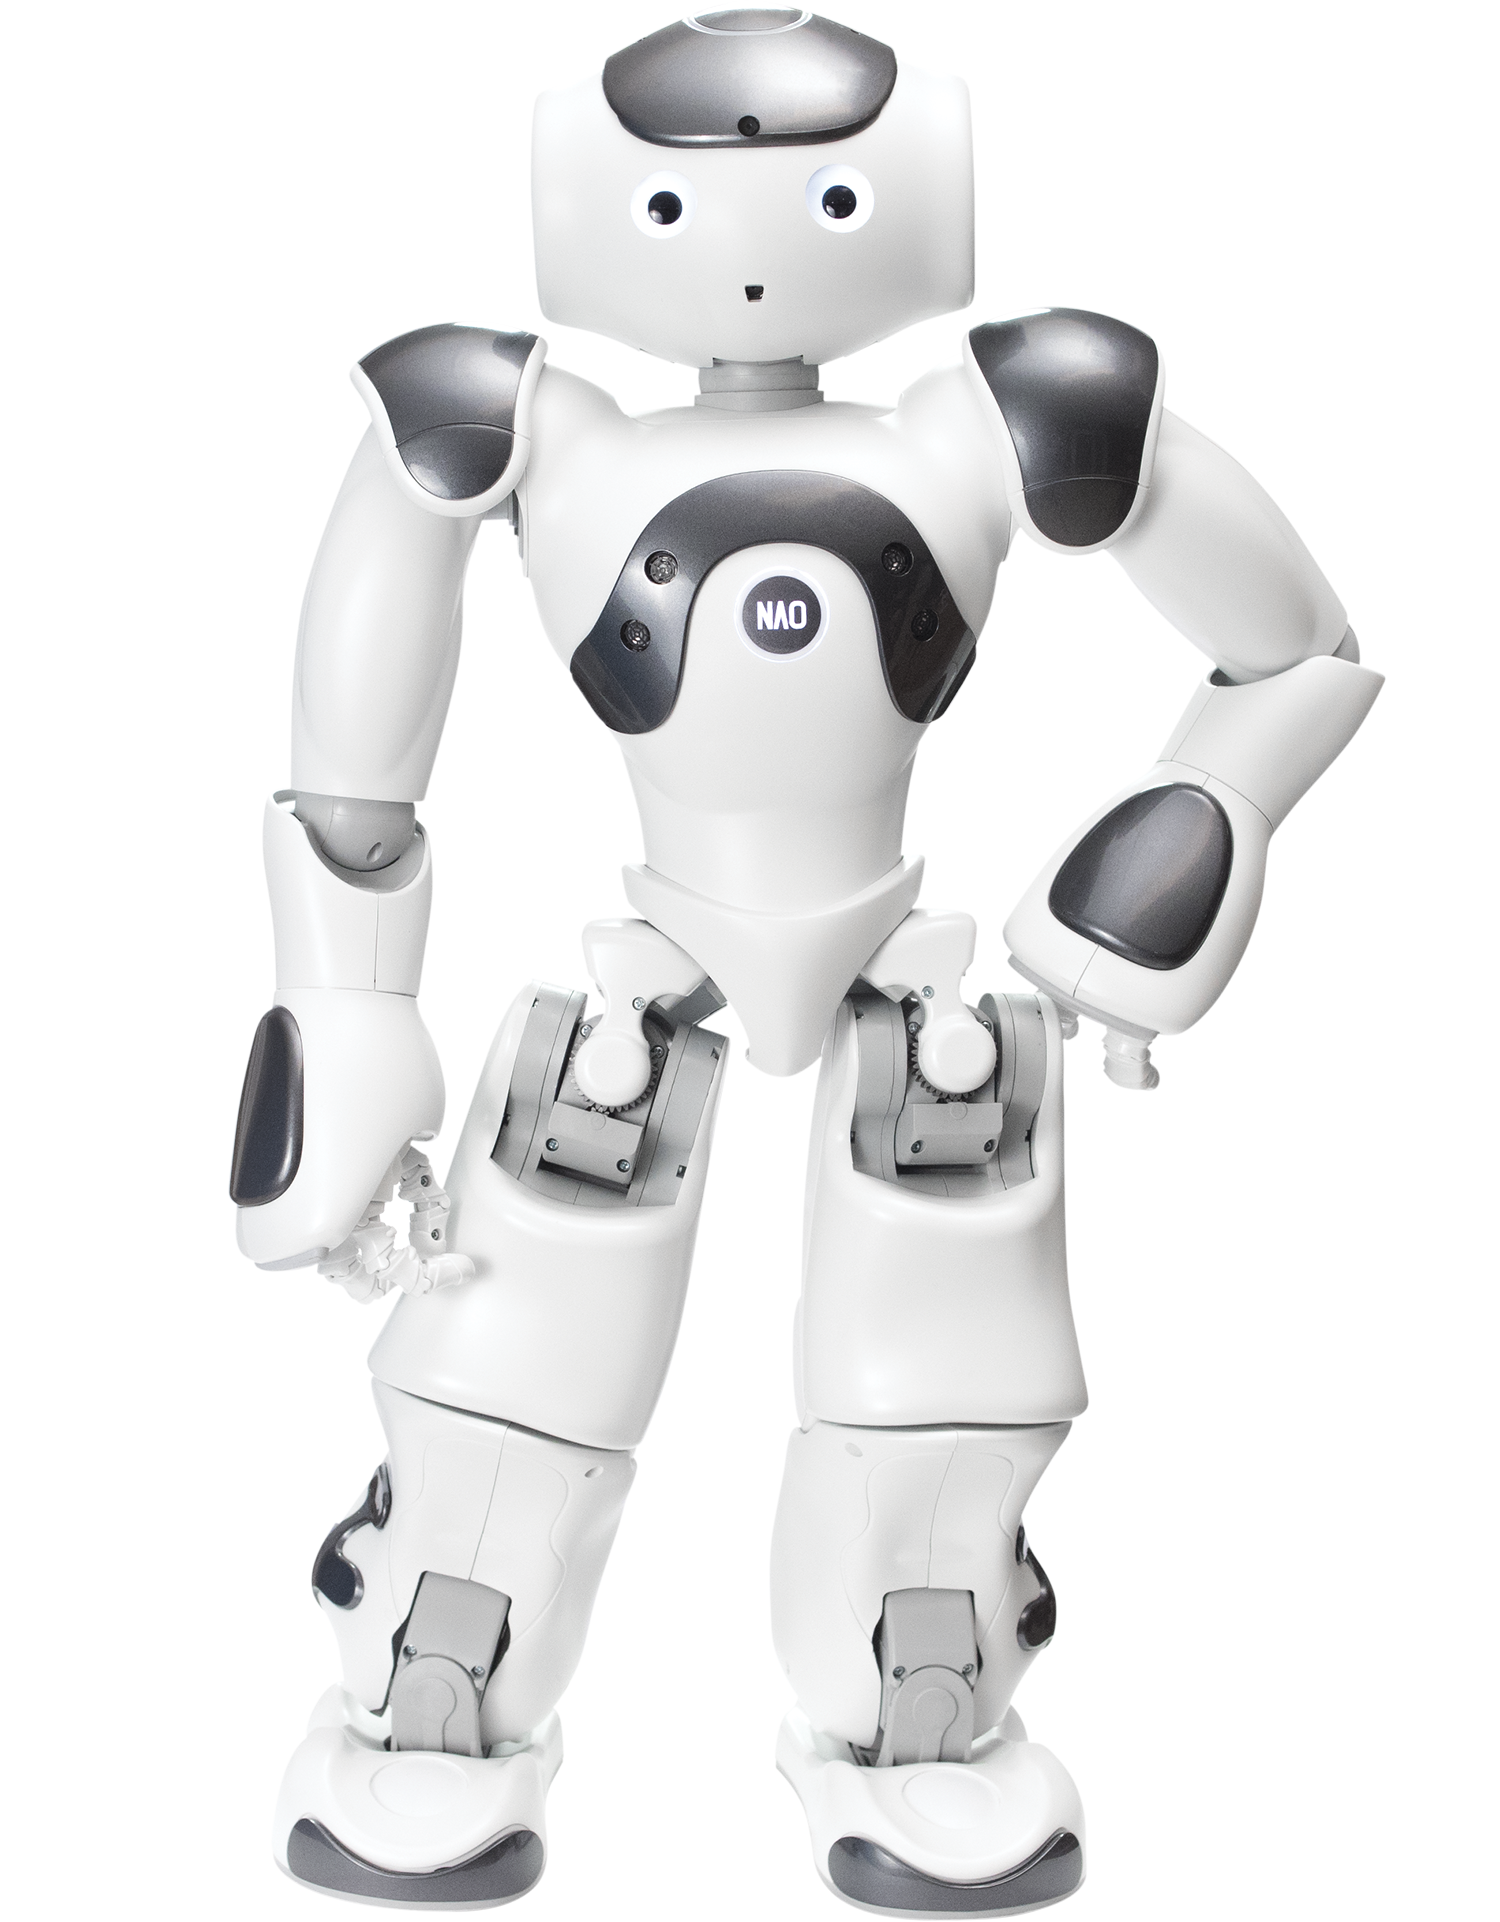
\includegraphics[width=\textwidth]{figures/NAO-v6.png}
    \caption{}
    \label{fig:nao-v6}
  \end{subfigure}
  \begin{subfigure}[b]{0.4\textwidth}
    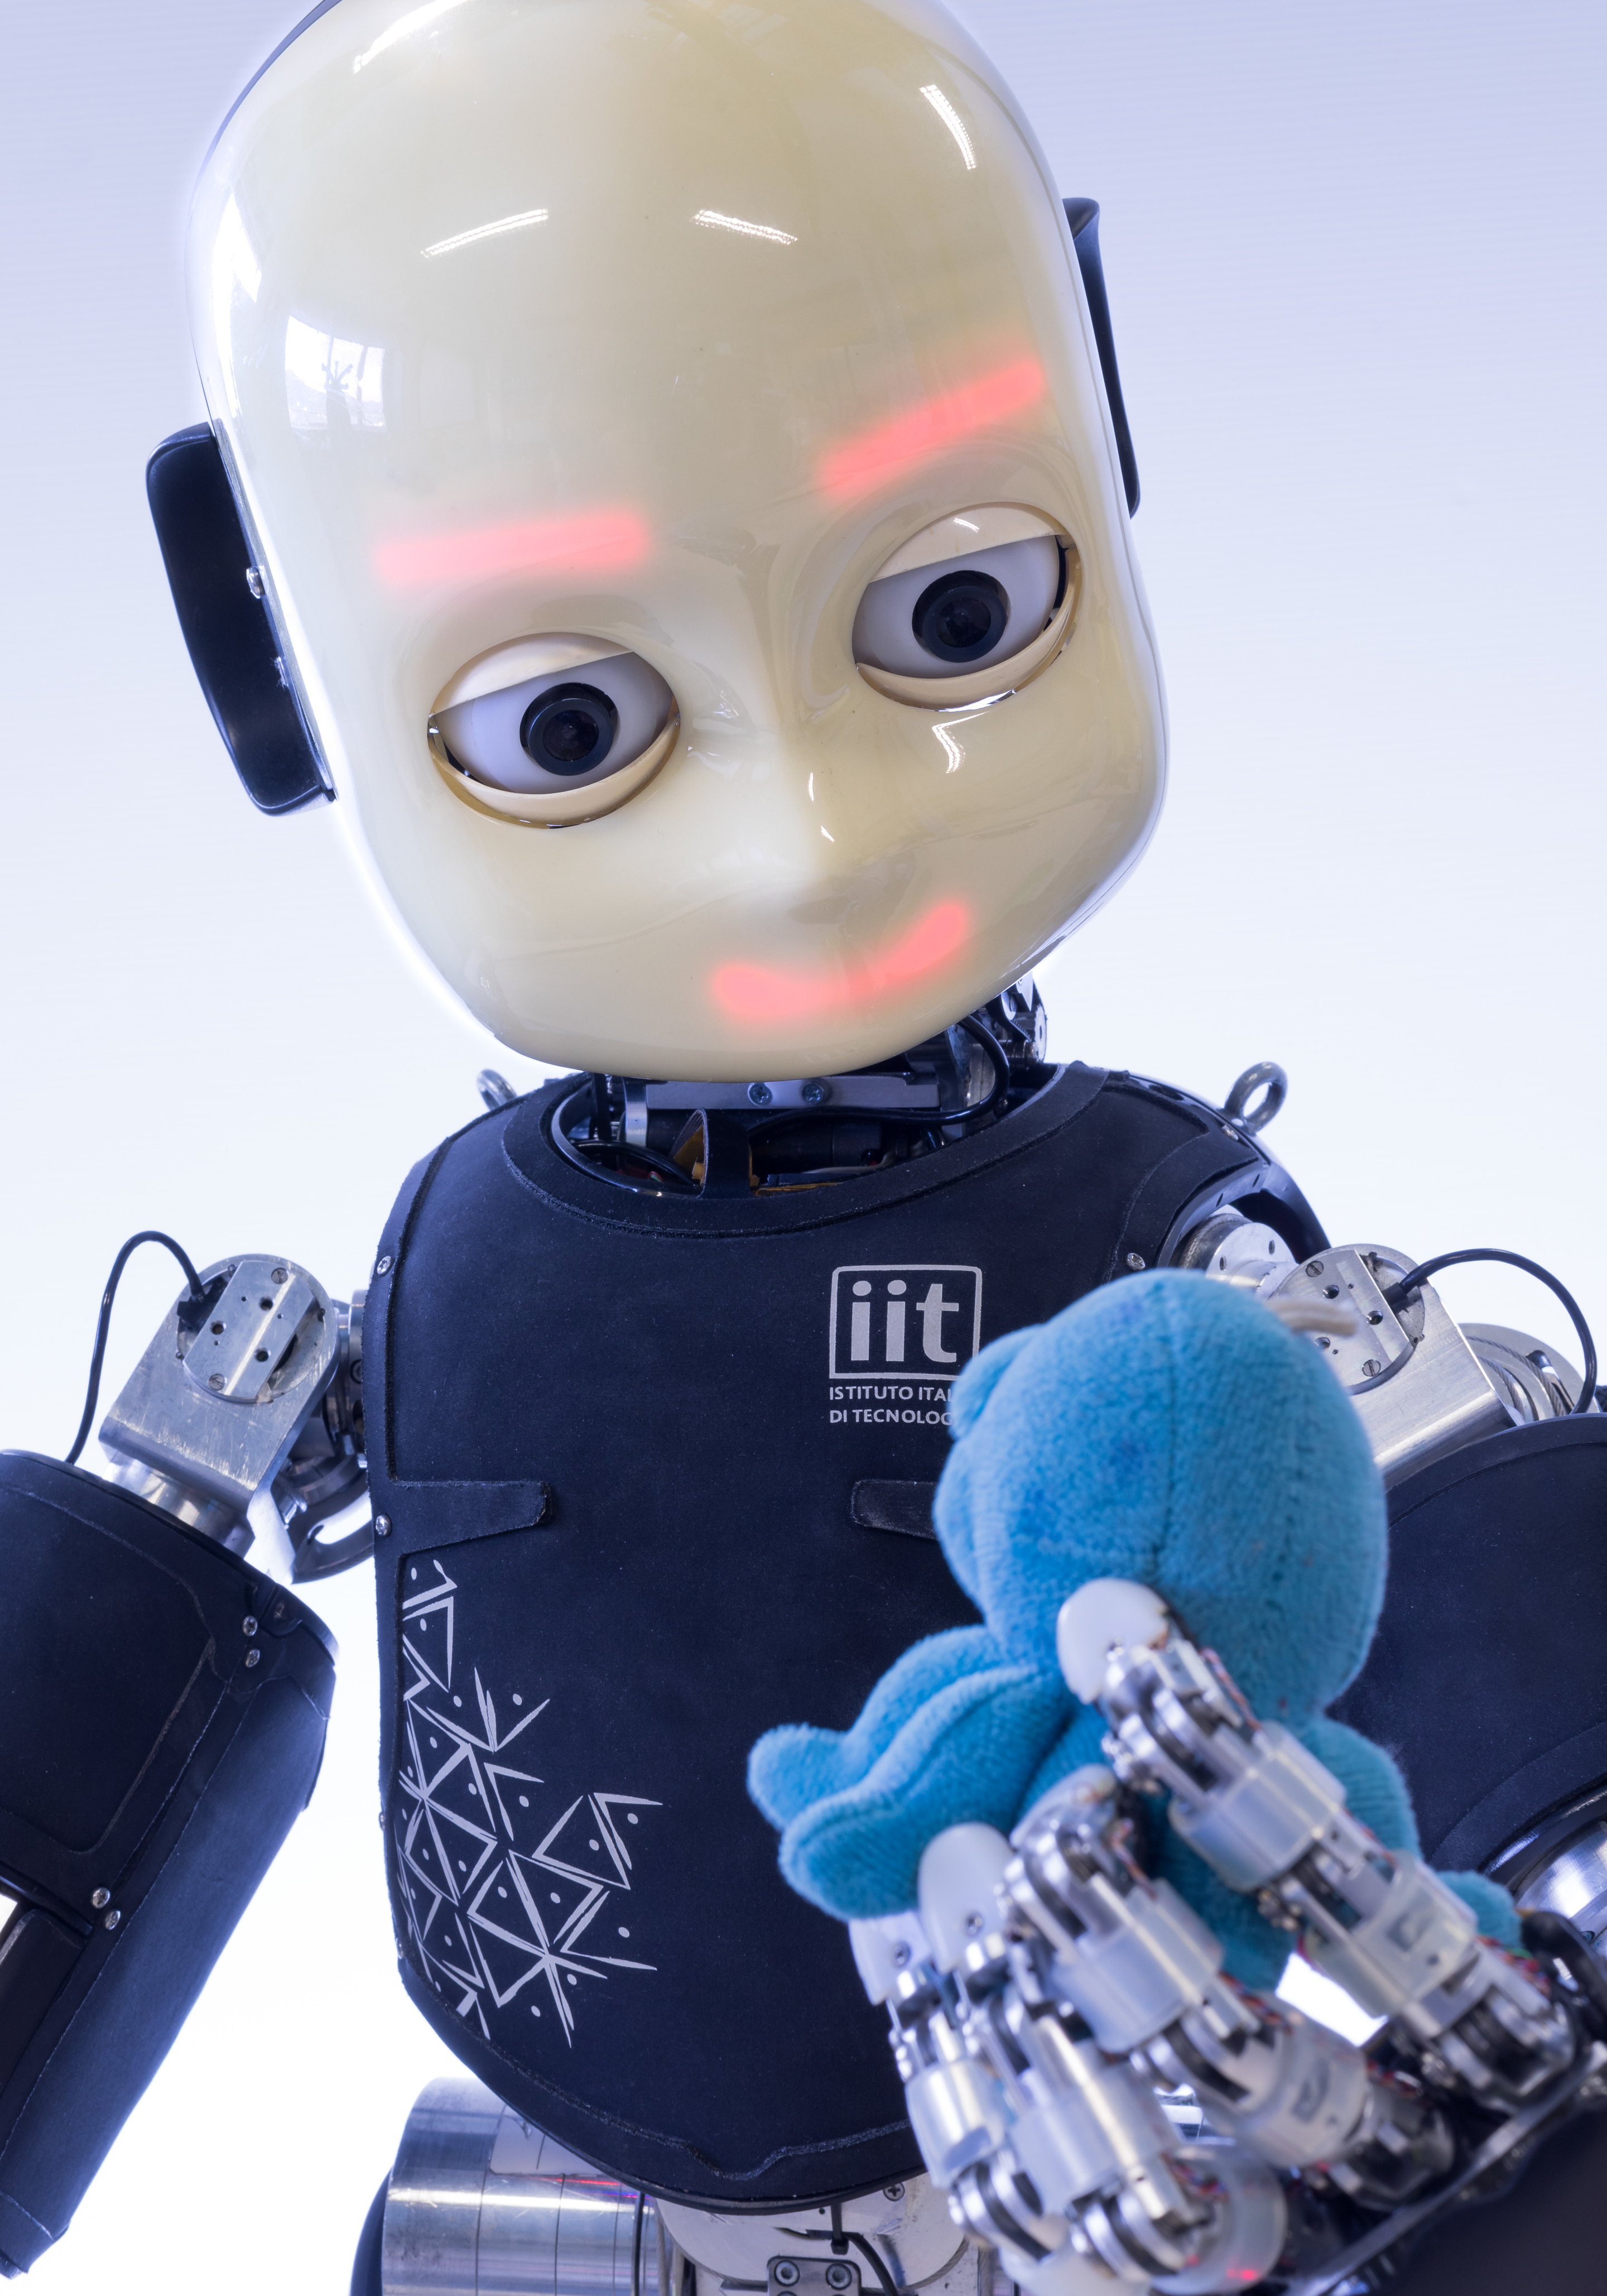
\includegraphics[width=\textwidth]{figures/iCub.jpg}
    \caption{}
    \label{fig:iCub}
  \end{subfigure}
  \caption{NAO v6 \cite{NAOdesign} on the left, used in RoboCup Standard 
      Platform League. iCub \cite{Sandini2007iCub} on the right, a cognitive 
      robotics research platform.}
\end{figure}

\begin{figure}
  \centering
  \begin{subfigure}[b]{0.4\textwidth}
    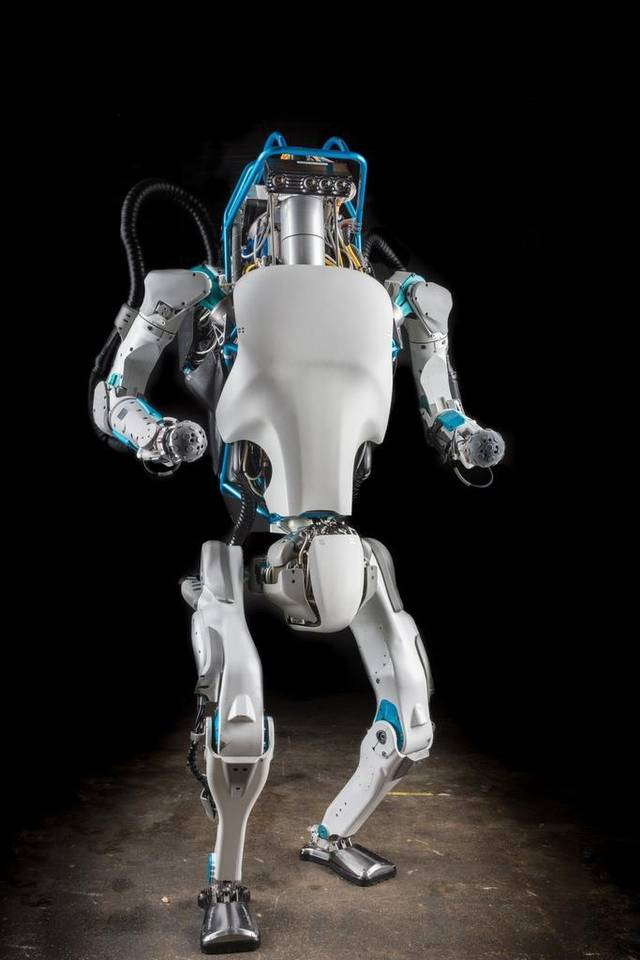
\includegraphics[width=\textwidth]{figures/ATLAS.jpg}
    \caption{}
    \label{fig:atlas}
  \end{subfigure}
  \begin{subfigure}[b]{0.4\textwidth}
    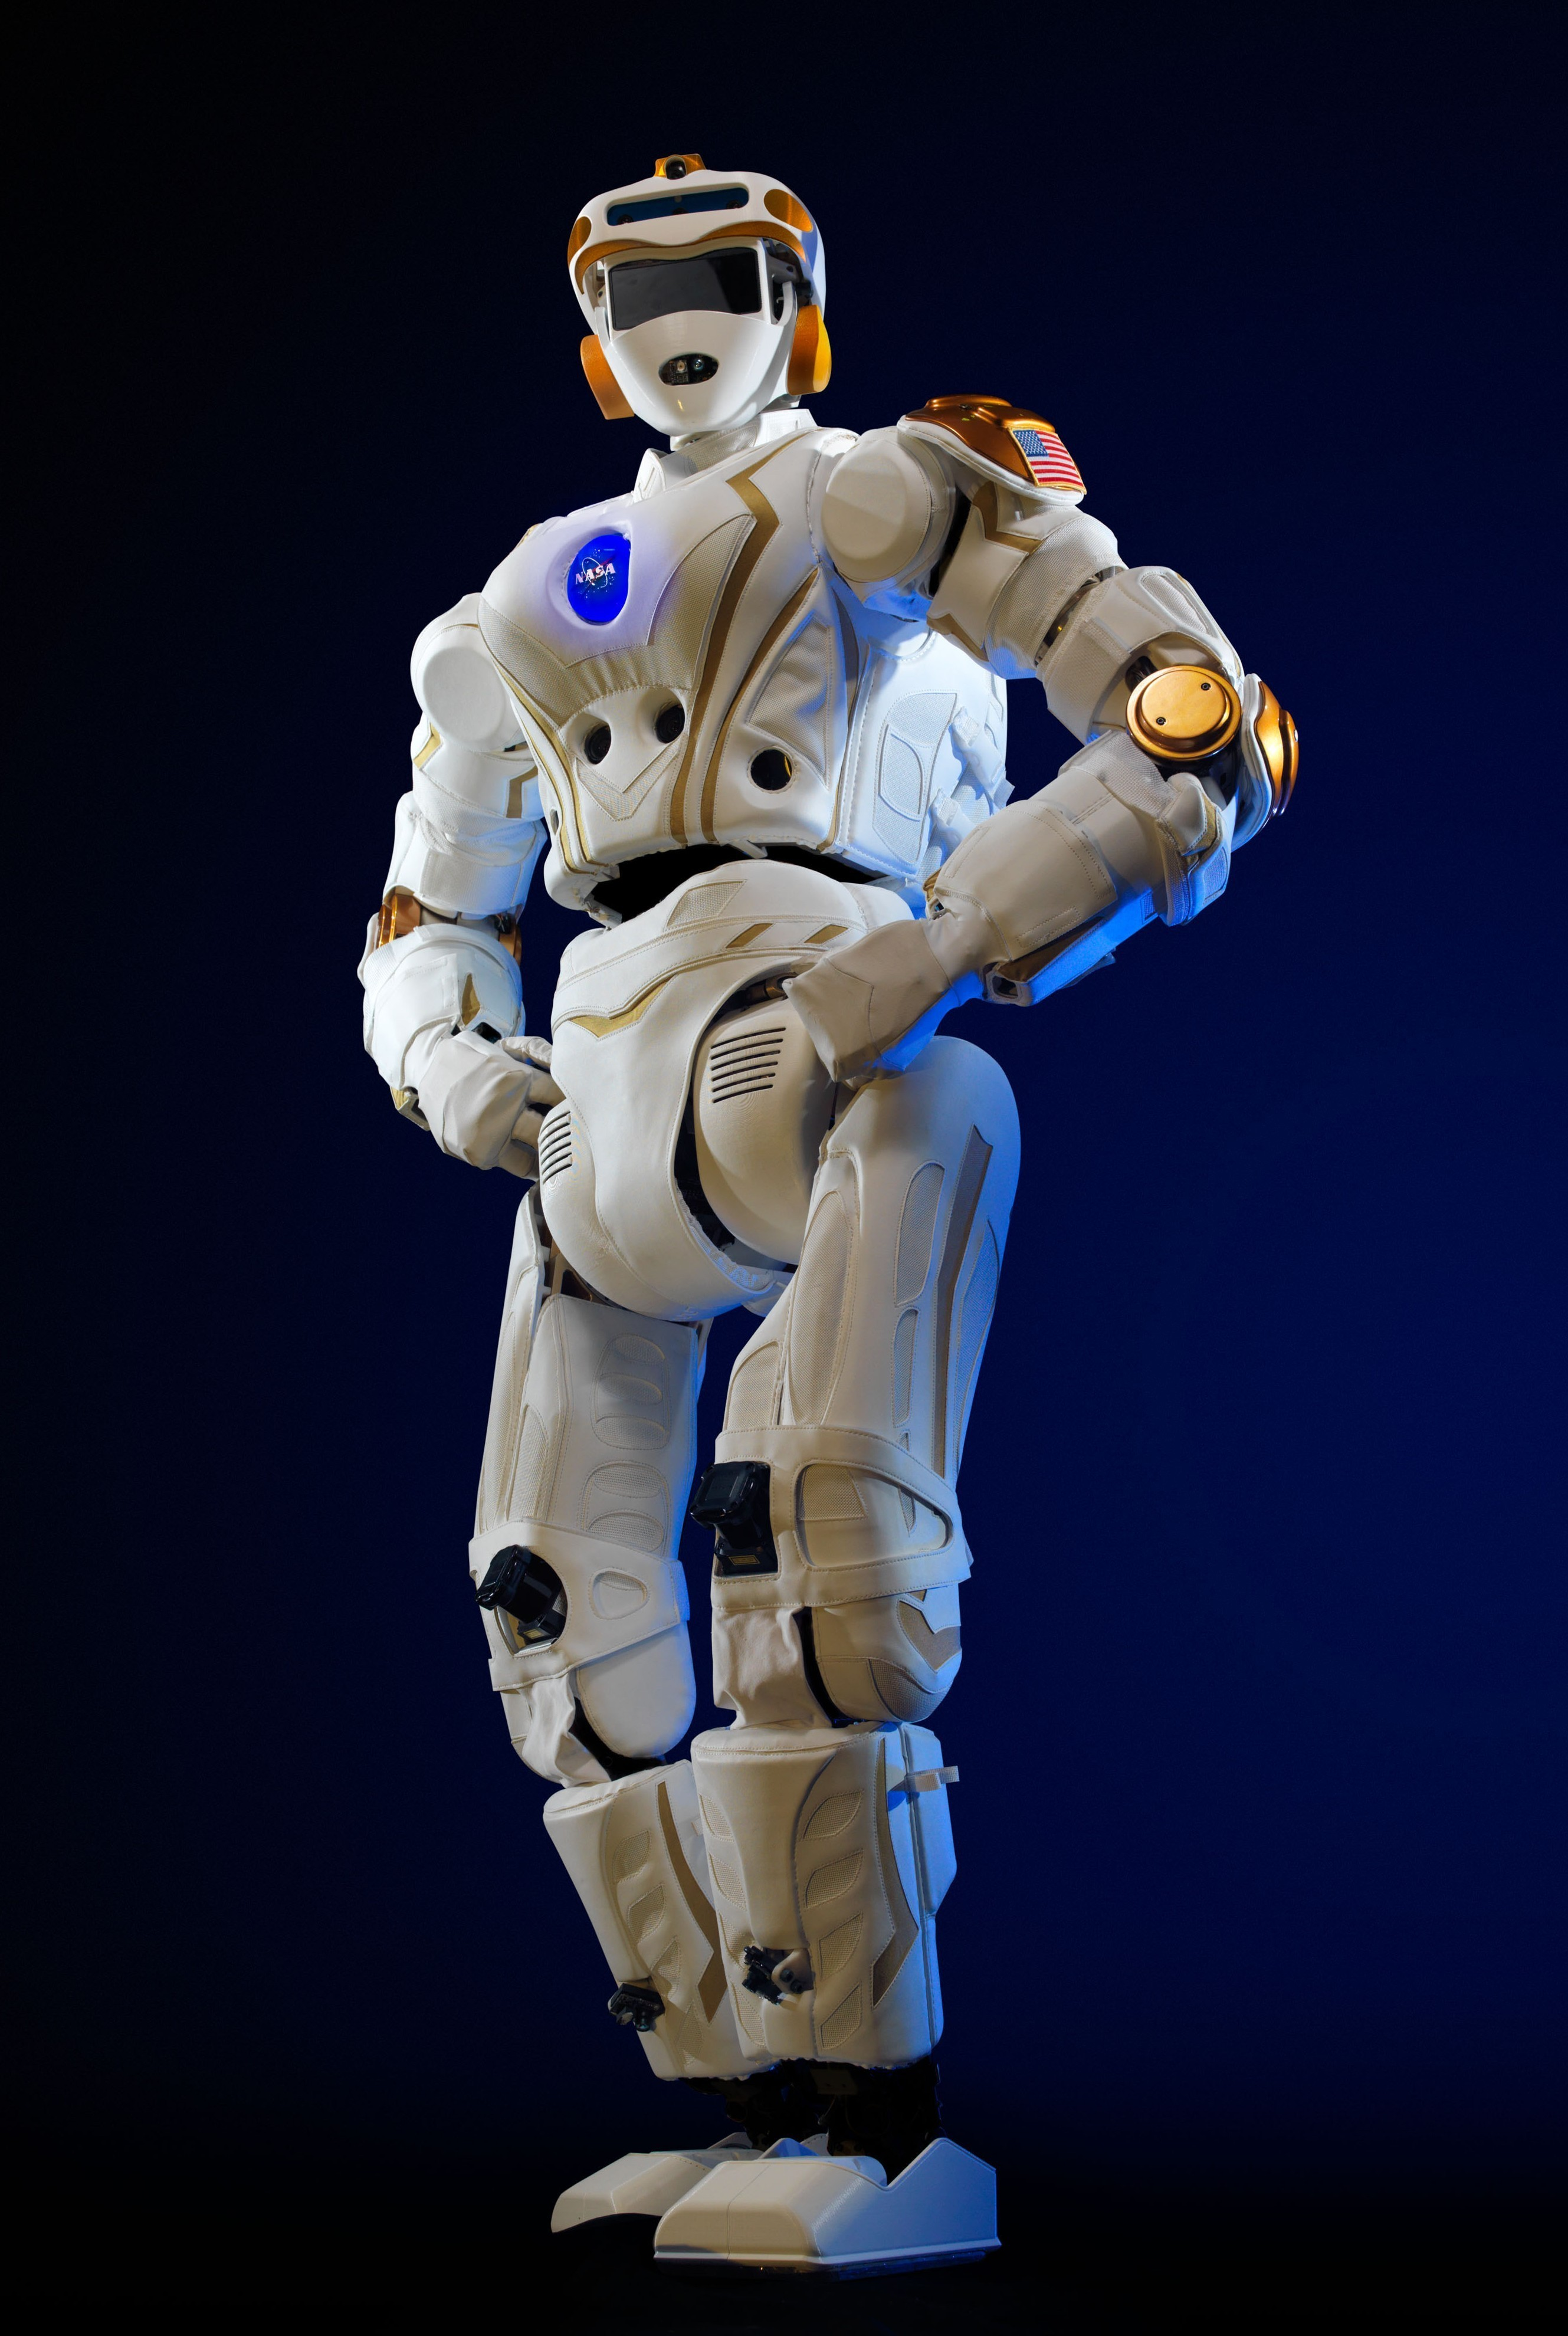
\includegraphics[width=\textwidth]{figures/NASA-Valkyrie.jpg}
    \caption{}
    \label{fig:valkyrie}
  \end{subfigure}
  \caption{ATLAS, on the left, and Valkyrie \cite{Radford2015Valkyrie}, on the 
      right, have been developed with the purpose of advancing rescue operations
      and space exploration missions.}
\end{figure}

\begin{figure}
  \centering
  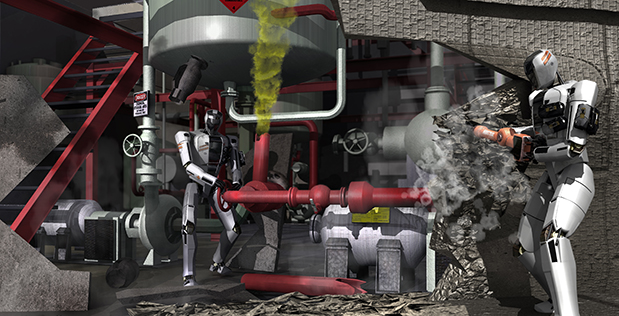
\includegraphics[width=\textwidth]{figures/DARPARoboticsChallenge.jpg}
  \caption{Typical scenarios described by DARPA Robotics Challenge
      \cite{Atkenson2018DARPARoboticsChallengeFinals}, where the human 
      intervention is dangerous and could put at risk life of rescuers.}
  \label{fig:drc}
\end{figure}

\section{Legged Robot Locomotion}
The problem of legged robot locomotion and its modules.

\begin{itemize}
  \item \textbf{Localization:} localization.
  \item \textbf{Mapping:} mapping. SLAM.
  \item \textbf{Planning:} planning.
  \item \textbf{Control:} control.
\end{itemize}

\section{Thesis Overview}
\textit{World of Stairs}. Aim of the thesis. NAO+xtion.
\texttt{elevation\_mapping}. Footstep planner (RRT).
Variable Height CoM IS-MPC. Block scheme.

Contributions: extending ECC19.
1. VH-CoM IS-MPC works on real robot.
2. Plan generated by planner works on real robot. Executed on external computer.
3. Introduction of \texttt{elevation\_mapping} into block scheme (directly
extending ECC19 scheme), allowing humanoid robot to move inside
\textit{World of Stairs} unknown environment.

Brief description of the results.

\begin{figure}
  \centering
  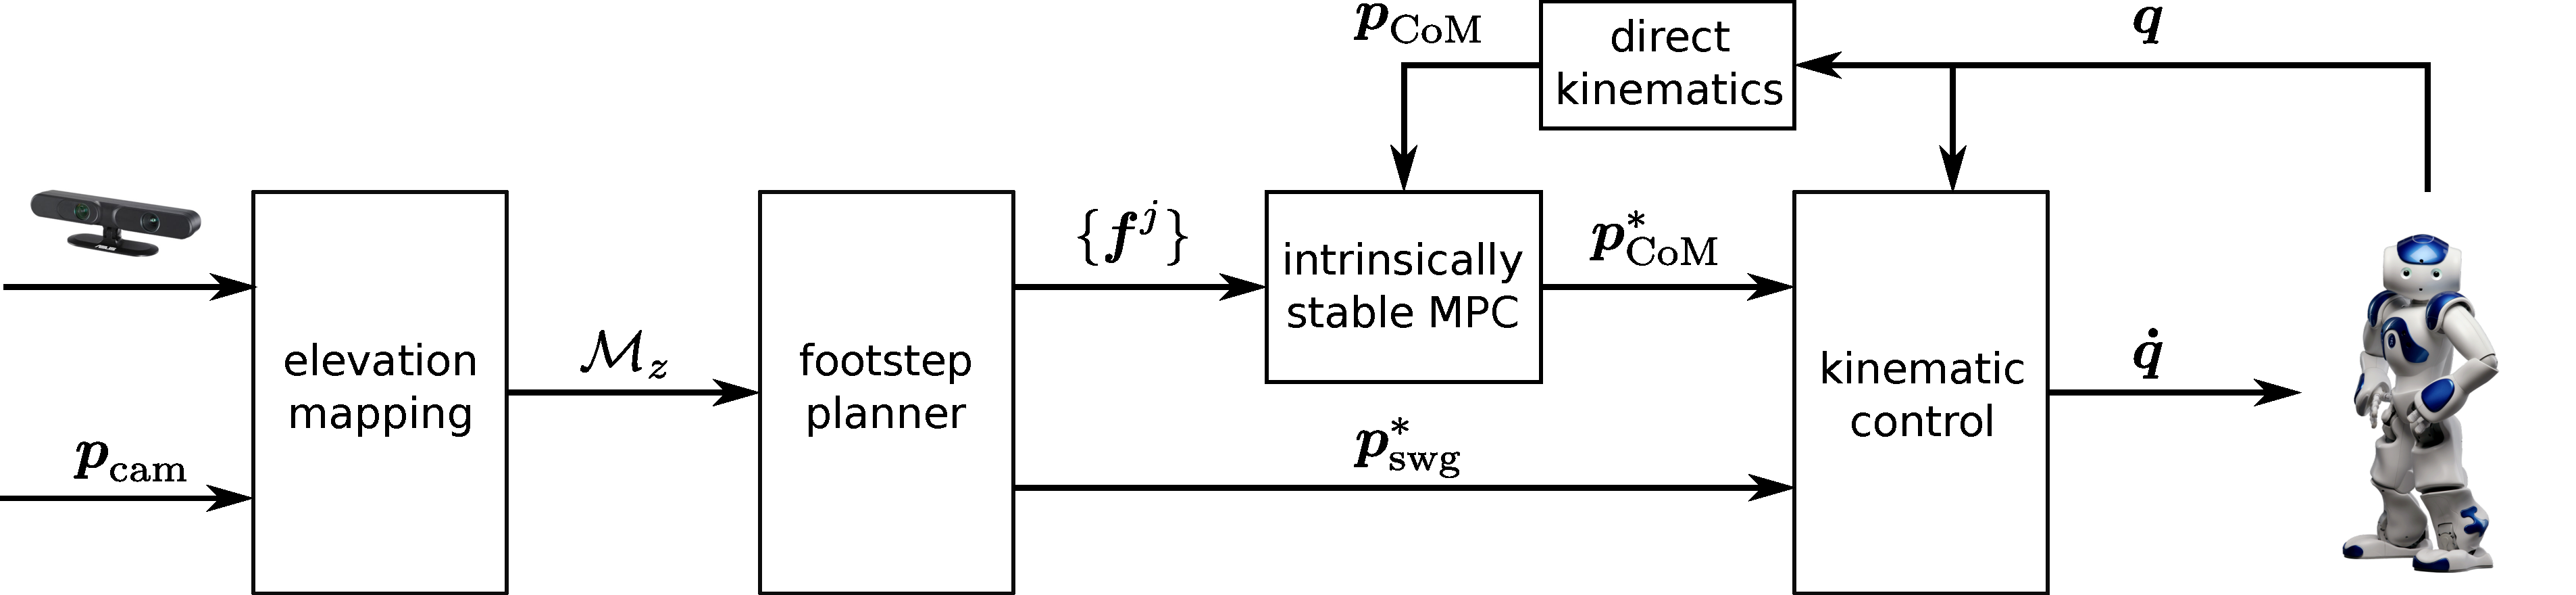
\includegraphics[width=\textwidth]{figures/BlockScheme.pdf}
  \caption{Block scheme of the approach.}
  \label{fig:block-scheme}
\end{figure}

